\newcommand{\SoftName}{GMemorise}
\newcommand{\HRule}{\rule{\linewidth}{0.5mm}}
\makeatletter
\g@addto@macro\@floatboxreset\centering
\makeatother

\documentclass[12pt,a4paper,twoside,openright]{book}
\usepackage[margin=2cm]{geometry}
\usepackage[pdftex]{graphicx}
\usepackage{graphviz}
\usepackage{amsmath}
\usepackage{float}
\usepackage{hyperref}
\usepackage[parfill]{parskip}
\usepackage[justification=centering]{caption}
\usepackage{url}
\usepackage{biblatex}
\usepackage{multirow}
\bibliography{thesis.bib}

\title{Predicting Responses to Spaced Repetition Flash Cards with Machine Learning Techniques}
\date{5 November, 2012}
\author{Jordan West}

\begin{document}
\frontmatter
% \maketitle
\begin{titlepage}

\begin{center}


% Upper part of the page

\includegraphics[width=0.8\textwidth]{./uqlogo.jpg}\\[1cm]    

\textsc{\Large Undergraduate Engineering Honours Thesis}\\[0.5cm]

\textsc{\LARGE Proposal}\\[0.5cm]


% Title
\HRule \\[0.4cm]
{ \Large \bfseries Measuring the Effectiveness of a Subset of Game Mechanics on Rote Memorisation of Foreign Vocabulary}\\[0.4cm]

\HRule \\[1.5cm]

% Author and supervisor
\begin{minipage}{0.4\textwidth}
\begin{flushleft} \large
\emph{Author:}\\
Jordan \textsc{West}
\end{flushleft}
\end{minipage}
\begin{minipage}{0.4\textwidth}
\begin{flushright} \large
\emph{Supervisor:} \\
Dr.~Mark \textsc{Schulz}
\end{flushright}
\end{minipage}

\vfill

% Bottom of the page
{\large \today}

\end{center}

\end{titlepage}


\cleardoublepage

\hfill Jordan West

\hfill 41184882

\hfill PO Box 6170 St Lucia QLD 4067

\vspace*{2cm}

5 November 2012

\vspace*{1cm}

Prof Paul Strooper \\
Head of School \\
School of Information Technology and Electrical Engineering \\
The University of\hspace{2pt}�Queensland \\
St Lucia QLD 4072 \\

Dear Professor Strooper, \\
In accordance with the requirements of Bachelor of Engineering (Honours) in the
School of Information Technology and Electrical Engineering, I hereby submit the following thesis entitled:

\vspace*{0.6cm}
\centerline{\textit{Predicting Responses to Spaced Repetition Flash Cards with Machine Learning Techniques}}
\vspace*{0.6cm}

The thesis was performed under the supervision of Dr. Mark Schulz. I declare that
the work submitted in this thesis is my own, except as acknowledged in the text and footnotes, and has
not been previously submitted for a degree at the University of Queensland or any other institution.


Yours sincerely,

\vspace*{2cm}

\rule{7cm}{0.2mm}

Jordan J. West

\chapter*{Acknowledgments}
This thesis would not have been possible without the support of my
supervisor Dr. Mark Schulz whose input and guidance
has been invaluable for the project.

I would like to thank Dr Yuriko Nagata for her assistance with this project and for allowing
me to introduce the software to her students. I would very much like to thank the students
of JAPN1023 who participated in the project, without whom none of this would have been possible.
I hope that the students found value in using the software.

I wish to acknowledge the help of Dr Michael Harrington of the School of Languages
and Comparative Cultural Studies
for his advice with additions to the online learning software.

I would also like to express my sincere appreciation to the UQ CEIT team for their
assistance with this project --
particularly the advice and guidance of Dr. Alan Cody and Prof. Phil Long.

Last but not least I want to thank my friends for their encouragement and
for putting up with me throughout the project, and finally Mum and Dad for being there
and without whose support, care and encouragement I would never have made it this far in
my university career.

\chapter*{Abstract}
With the development of personal computers and smart phones, many new learning environments 
and learning methods are emerging. With this, educational data collection has become
 trivial and is becoming a powerful tool for improving education. This project created
 an online flash-card environment for memorising foreign vocabulary, and attempted to 
 predict whether a student will be able to recall a particular word in a target language 
 by tracking, recording and analysing reviews with machine learning techniques. 
This has many implications in education, including identifying struggling students,
identifying difficult
vocabulary to focus on, as well as improving methods of memorisation of foreign
vocabulary.
 The web based software was available from desktop and mobile devices and allowed
 students to study anywhere. Over 13 weeks, 28 students 
 completed over 7,500 reviews. The results were promising, with the system correctly 
predicting student recall of approximately 70\% of flash-card reviews. The rate of forgetting was
also plotted based on the review data, however the amount of data and number of 
reviews was too small
for any significant findings. Future work might involve a larger number of more motivated
students to gather a larger dataset.


\newpage

\tableofcontents

\mainmatter
The recent proliferation of addictive game-like features (or \textit{game mechanics}) to 
increase user engagement in non-game environments such as social networks and 
sales websites raises the question: 
How effective could game mechanics be when applied in other environments, such as 
education? This project aims to construct software and analyse and quantify the
effectiveness of the application of a subset of game mechanics to an online 
learning environment in motivating and engaging students. Specifically for 
this project the learning environment selected is the memorisation of vocabulary 
of a foreign language.

\subsubsection{Game Mechanics} \label{background_gamemechanics}
\subsubsection{Extrinsic vs. Intrinsic Motivation}
Motivation is often seperated into two categories - Extrinsic and Intrinsic motivation. Intrinsic motivation refers to the motivation one feels for a task when that person feels that completing the task is enjoyable or fulfilling. Extrinsic motivation 
\subsubsection{socialPsych}
The socialPsych\cite{landers_casual_2011} project examined some game mechanics
in an online social learning environment which was run in parallel to university
courses. The authors of the project compiled a list of best practices
for casual social games used for learning, of which a few are relevant to
the project discussed in this proposal. Immediacy of feedback (in terms of
rewards or validation for completing a task) was found to be important for
motivation \cite[p. 419]{landers_casual_2011}. Game rewards should also be adjusted
to a difficulty which is achievable without being overly easy to ensure the user
feels satisfaction upon completion \cite[p. 420]{landers_casual_2011}.

The system will be deployed for use by students enrolled in a Japanese course at
The University of Queensland.

Users will be randomly assigned to one of two groups - Group A or Group B. Group
A will use a learning environment with a series of learning modules and tests,
while Group B will use the same learning environment with the addition of some 
game mechanics. At no point will users be required to carry out any task for
assessment or otherwise, and users may opt-out and delete all their data at
any time.

The actions of the students will be logged over a six-week period during which
the system will be available to them. Specifically which actions will be logged
is discussed in section \ref{scope_datacollection}. These actions will be 
analysed to determine the engagement of the users in each group.

\chapter{Results}
\section{Usage Statistics}

A total of 28 students registered to use the software and 7,879 total reviews were recorded
by 3 November 2012.

Students showed interest in the software during the in-class introduction, however many
students registered and used the software only once. Figure \ref{fig_visits} shows the initial
interest in the software as a spike in the number of visits toward the beginning of semester.
This graph tracks all visits including users that have not yet registered.

\begin{figure}[h!]
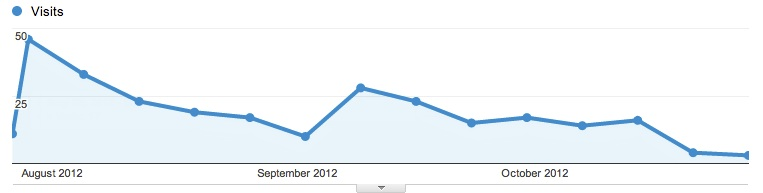
\includegraphics[width=12cm]{img/visits.jpg}
\caption{Google Analytics data on total number of visits to the application}
\label{fig_visits}
\end{figure}

Figure \ref{fig_usage_devices} shows most students accessed the software from a
desktop computer, while a handful accessed the
software exclusively from a mobile device. A single user accessed the software from both
a desktop and mobile device.

\begin{figure}[h!]
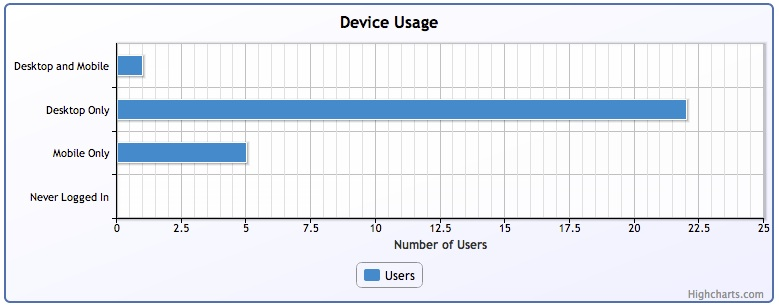
\includegraphics[width=12cm]{img/usage_devices.jpg}
\caption{The number of users according to the device used to access the software.}
\label{fig_usage_devices}
\end{figure}

The number of reviews completed per user is one of the more important statistics as
it shows the diversity of `useful' review data. Too many first reviews are useless as
they contain no useful data on which to later predict an answer.
Figure \ref{fig_usage_reviewcount} shows that eight users completed only new
reviews (the 1-20 range) after registering.

For the purposes of the following graphs, users were classified as `active' or `inactive'
based on the number of total reviews completed, with active users considered as those
who completed more than 200 reviews.

\begin{figure}[h!]
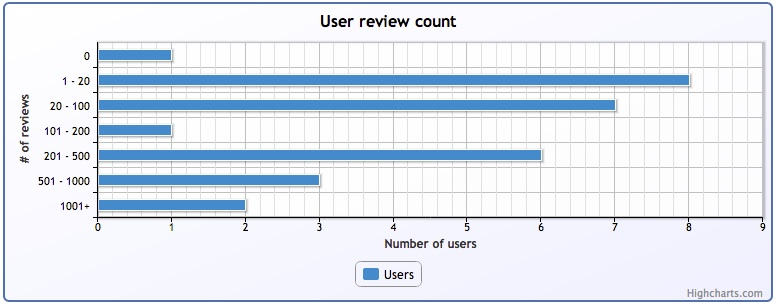
\includegraphics[width=12cm]{img/usage_reviewcount.jpg}
\caption{Number of users per total reviews. Users who had completed 
at least 200 reviews were considered `active users'.}
\label{fig_usage_reviewcount}
\end{figure}

Figure \ref{fig_usage_semester} shows the average number of reviews per user across the
semester. Users were divided up into `active' and `inactive' groups to avoid inactive
users skewing the data, though an average across all users is also shown with the blue line.

\begin{figure}[h!]
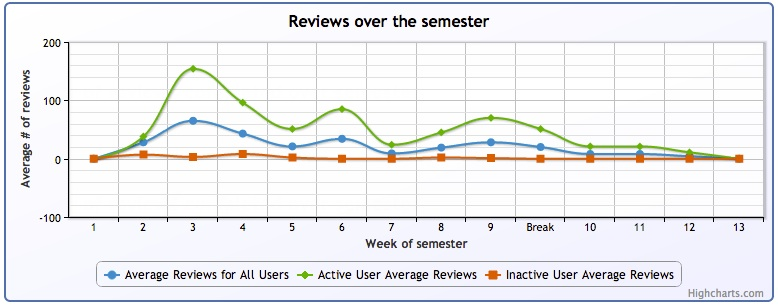
\includegraphics[width=12cm]{img/usage_semester.jpg}
\caption{Usage of the system over the semester.}
\label{fig_usage_semester}
\end{figure}

Users tended to complete the most reviews on their first day after registering.
Figure \ref{fig_usage_sinceregistering} groups
reviews by the number of days since registering, showing a very fast decline in
number of reviews in the first couple of weeks after registering.

\begin{figure}[h!]
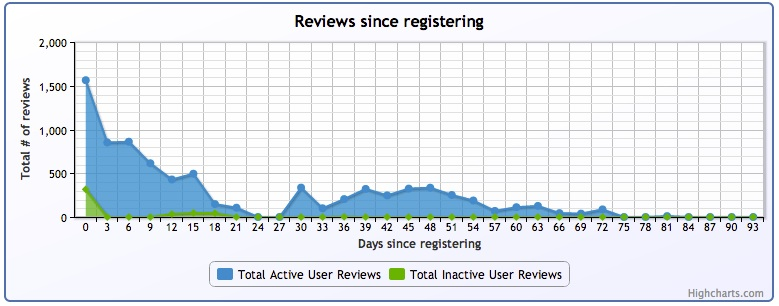
\includegraphics[width=12cm]{img/usage_sinceregistering.jpg}
\caption{Usage of the system shown as the number of days since registering.}
\label{fig_usage_sinceregistering}
\end{figure}

Figure \ref{fig_usage_sinceregistering} shows the total number of reviews per user
after registering. Only a few users registered in the second week of semester,
 with many more registering in the following weeks. However many users only
 completed reviews in the first few days after registration and stopped usage after
 that.
 
Only a few users used the software regularly; table \ref{tbl_topusers} shows the
statistics for the top five users by number of reviews.

\begin{table}[h!]
\caption{Top users and study statistics}
\label{tbl_topusers}
\begin{tabular}{|c|c|c|c|}
\hline
User ID & Number of logins & Vocabulary studied & Total reviews \\
\hline
20 & 59 & 100\% & 1910 \\
10 & 13 & 75\% & 1337 \\
21 & 13 & 45\% & 831 \\
19 & 9 & 50\% & 781 \\
26 & 9 & 58\% & 718 \\
\hline
\end{tabular}
\end{table}

\section{User Demographics}

\begin{table}[h!]
\caption{Gender of registered users}
\begin{tabular}{|c|c|}
\hline
Gender & No. of users \\
\hline
Male & 7 \\
Female & 21 \\
\hline
\end{tabular}
\end{table}

\begin{table}[h!]
\caption{Native language of registered users}
\begin{tabular}{|c|c|}
\hline
Native language & No. of users \\
\hline
English & 21 \\
Other & 7 \\
\hline
\end{tabular}
\end{table}

\section{Forgetting Curves}
\subsection*{Generated from Recorded Reviews}

Figure \ref{fig_expforgetcurve} shows the review data grouped
as data points by the review number and days since previous review (actual interval).
The threshold $n$
is the number of reviews required for a data point to be displayed.

The progression from $n \geq 5$ to $n \geq 100$ shows a significant reduction of noise
in the data points, where $n$ is the number of reviews required to generate a single data
point. Ideally this threshold would be much higher, however with the limited data set
available increasing the threshold any more would reduce the number of data points
visible.

\begin{figure}[h!]
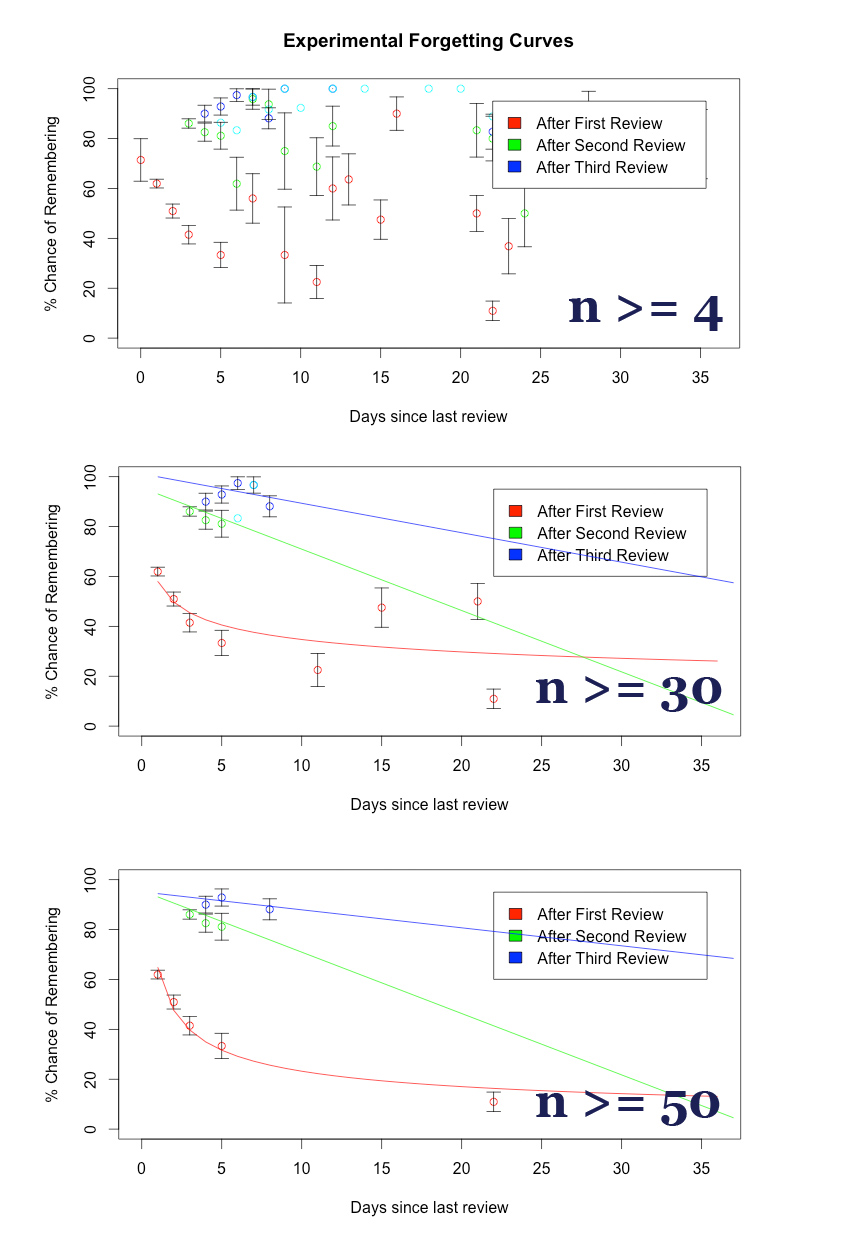
\includegraphics[width=14cm]{img/forgettingcurves.jpg}
\caption{Forgetting curves produced from recorded review data with various thresholds
for number of reviews required to generate a data point}
\label{fig_expforgetcurve}
\end{figure}

A much larger number of reviews were available for the first review, so the standard error
is reduced. The standard error as shown on the $n \geq 30$
graph in figure \ref{fig_expforgetcurve} for the first
data point is 1.7\% with the chance of remembering calculated from $n = 774$ review samples.
In contrast, the data point at fifteen days for the first review was calculated from only 
$n = 40$ available review samples, and has a standard error of 7.9\%.

Equation \ref{eqn_forgetcurvefit} shows the curve that was fitted to the data for recall
after the first review, while equations \ref{eqn_forgetcurvefit2} and \ref{eqn_forgetcurvefit3}
show the lines fitted to the data for recall after the second and third reviews respectively.

\begin{equation}
\label{eqn_forgetcurvefit}
P = \frac{x^{-0.4466}}{0.0154}
\end{equation}

\begin{equation}
\label{eqn_forgetcurvefit2}
P = -2.46x + 93.1
\end{equation}

\begin{equation}
\label{eqn_forgetcurvefit3}
P = -0.72x + 94.4
\end{equation}

\section{Prediction of Recall}

The machine learning algorithms tested averaged just under 70\% accuracy, with
the best performance on the validation set by the radial kernel based support vector
machine at 70.1\%.

Table \ref{tbl_algo_comparison} lists the algorithms tested and the accuracy of
classification on both the training and validation sets.

\begin{table}[h!]
\caption{Comparison of the performance of various machine learning algorithms on the output `Correct'. Accuracies are averaged over 15 runs.}
\label{tbl_algo_comparison}
\begin{tabular}{|p{5cm}|c|c|}
\hline
Algorithm & Training set accuracy & Validation set accuracy \\
\hline
Linear SVM & 69.41\% & 68.92\% \\
Radial SVM & 71.55\% & 70.14\% \\
Neural Network (Linear, 9 hidden units) & 72.65\% & 69.34\% \\
\hline
\end{tabular}
\end{table}

\begin{table}[h!]
\caption{Confusion matrix of SVM Radial Kernel on validation data with output `Correct'}
\label{tbl_confusionmatrix_correct}
\begin{tabular}{|cc|cc|}
\hline
& & \multicolumn{2}{|c|}{Actual} \\
 & & Incorrect & Correct \\
\hline
\multirow{2}{*}{Predicted} & Incorrect & 742 & 460 \\
& Correct & 321 & 1008 \\
\hline
\end{tabular}
\end{table}

\begin{table}[h!]
\caption{Confusion matrix of SVM Radial Kernel on validation data with output `User Rated Answer'}
\label{tbl_confusionmatrix_ura}
\begin{tabular}{|cc|cccccc|}
\hline
& & \multicolumn{6}{|c|}{Actual} \\
 & & 0 & 1 & 2 & 3 & 4 & 5 \\
\hline
\multirow{6}{*}{Predicted} & 0 & 104 & 54 & 34 & 47 & 25 & 43 \\
& 1 & 48 & 155 & 76 & 98 & 48 & 40 \\
& 2 & 44 & 100 & 217 & 101 & 109 & 78 \\
& 3 & 3 & 37 & 9 & 156 & 55 & 12 \\
& 4 & 9 & 43 & 48 & 77 & 151 & 69 \\
& 5 & 11 & 21 & 50 & 31 & 62 & 266 \\
\hline
\end{tabular}
\end{table}


\chapter{Discussion}
\section{Changes to Original Scope}
* Removed testing and scoring tests
* Removed typed answers, self evaluation only
\section{Evaluation}
\subsection{Usage of Software}
\subsection{Prediction of Recall}
\section{Potential Future Work}
* Vary the reschedule date slightly from the interval so that data is available for more
than just the common intervals



%\bibliographystyle{plain}
%\bibliography{thesis}
\printbibliography

\appendix
\chapter{Participant Information Sheet}
\label{appendix_participant_info_sheet}
\newpage
\fbox{
\includegraphics[page=1,width=17cm]{appendix/participant_info_sheet.pdf}}
\chapter{Participant Consent Form}
\newpage
\label{appendix_participant_consent_form}
\fbox{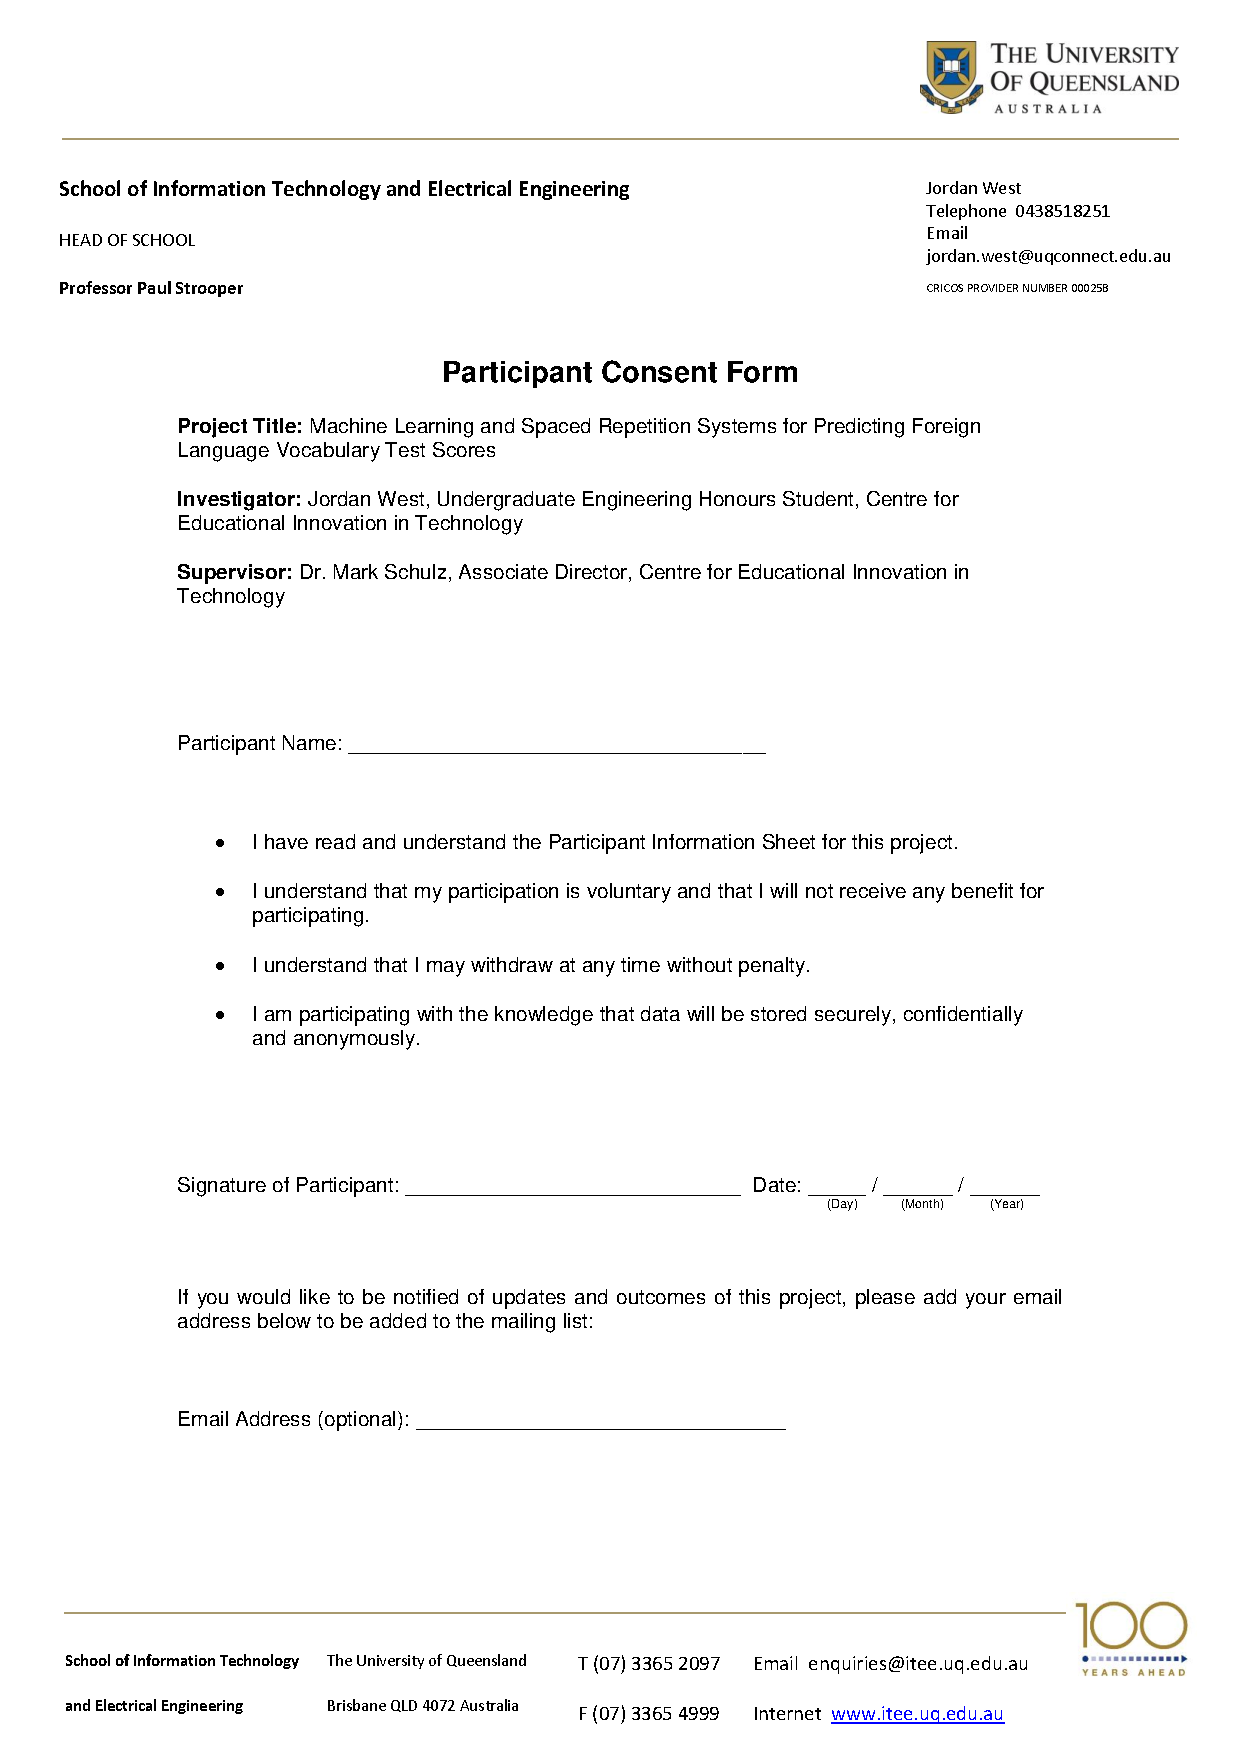
\includegraphics[page=1,width=17cm]{appendix/participant_consent_form.pdf}}
\chapter{Original Wireframes}
\newpage
\label{appendix_wireframes}

\fbox{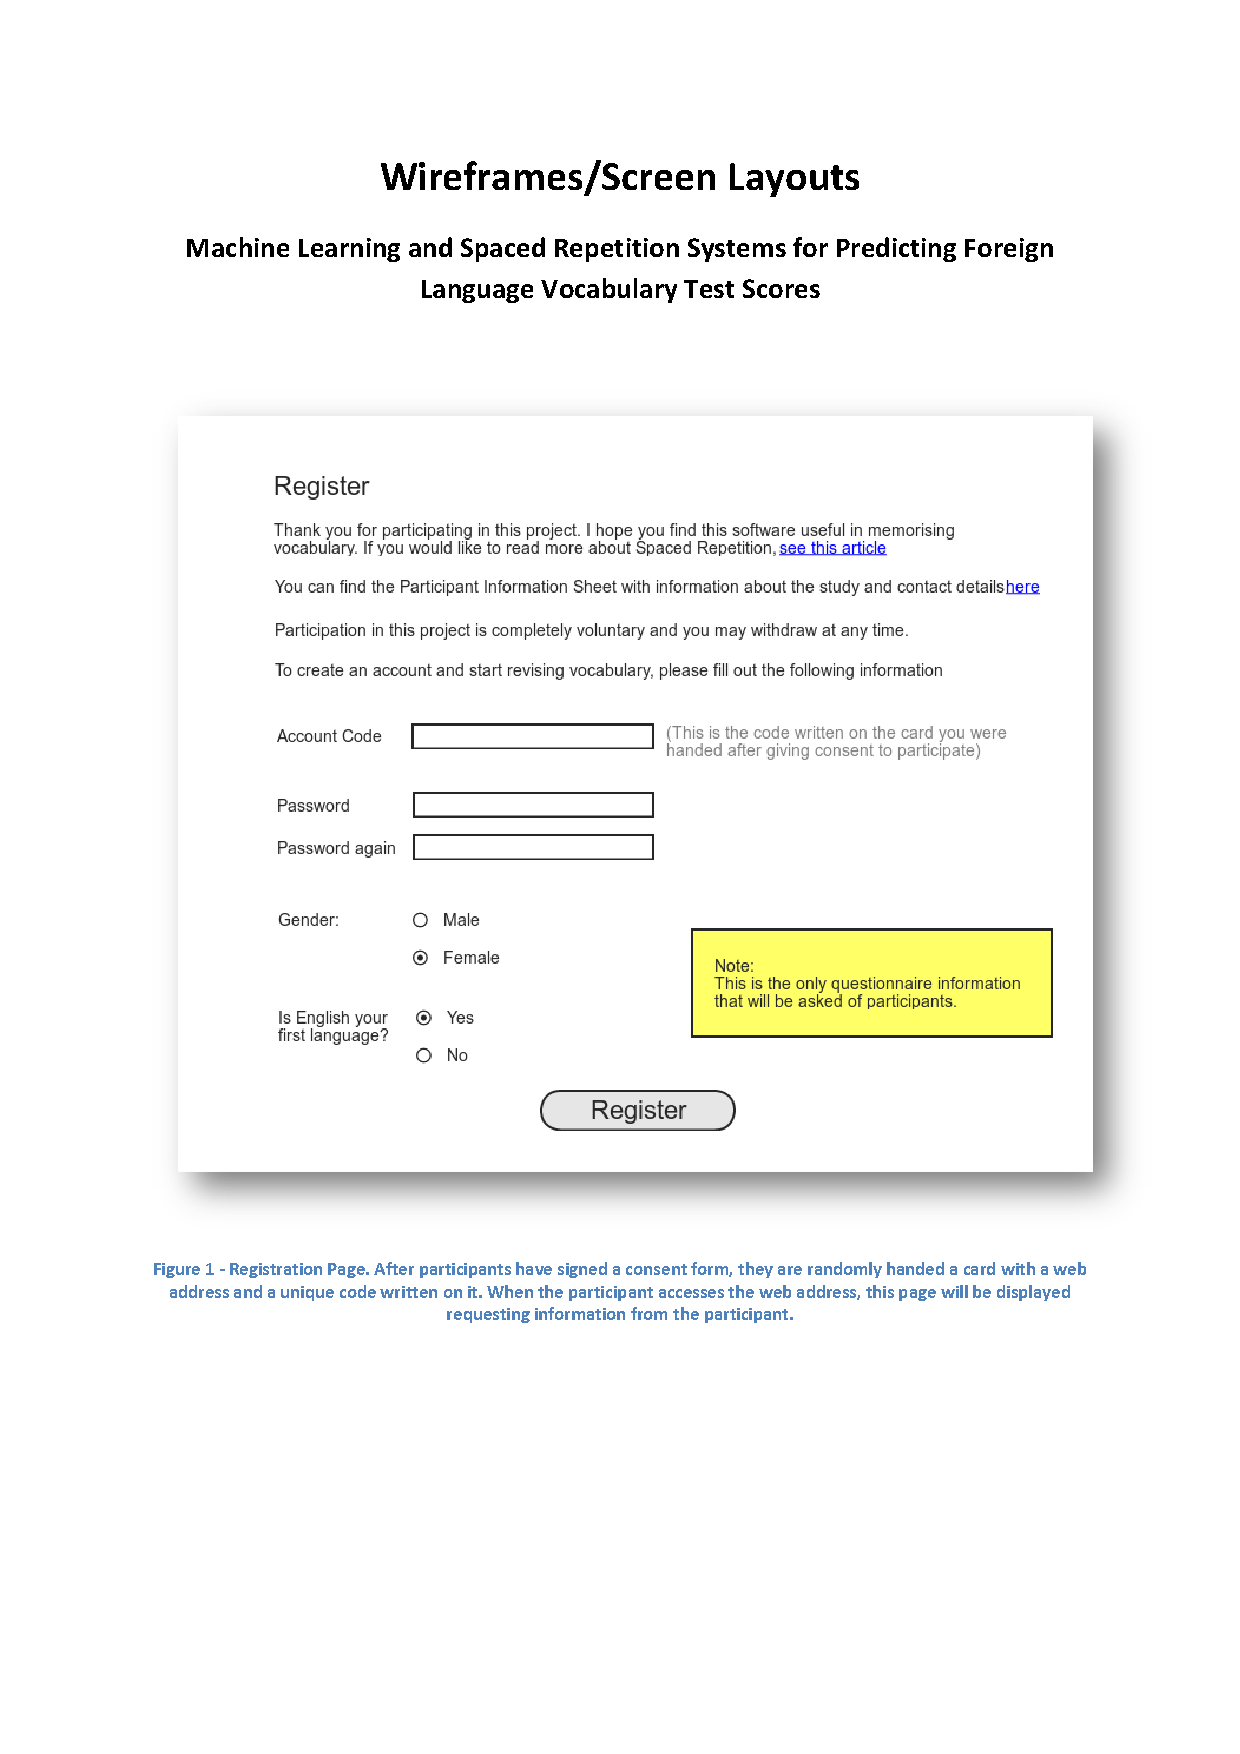
\includegraphics[page=1,width=17cm]{appendix/wireframes.pdf}}\newpage
\fbox{\includegraphics[page=2,width=17cm]{appendix/wireframes.pdf}}\newpage
\fbox{\includegraphics[page=3,width=17cm]{appendix/wireframes.pdf}}\newpage
\fbox{\includegraphics[page=4,width=17cm]{appendix/wireframes.pdf}}\newpage
\fbox{\includegraphics[page=5,width=17cm]{appendix/wireframes.pdf}}\newpage
\fbox{\includegraphics[page=6,width=17cm]{appendix/wireframes.pdf}}

\chapter{Membit Screenshots}
\label{appendix_screenshots}

\begin{figure}[h!]
\fbox{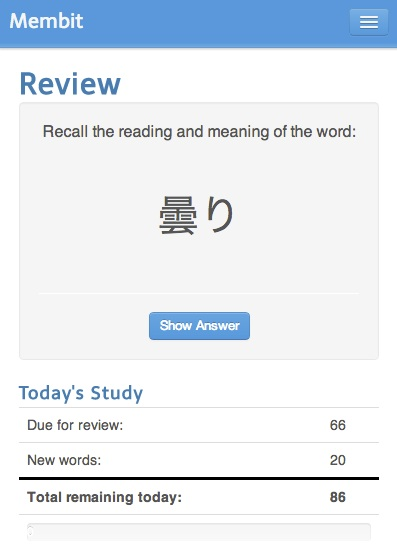
\includegraphics[width=7cm]{appendix/screenshots/mobile_review.jpg}}
\caption{Mobile review interface}
\end{figure}

\begin{figure}[h!]
\fbox{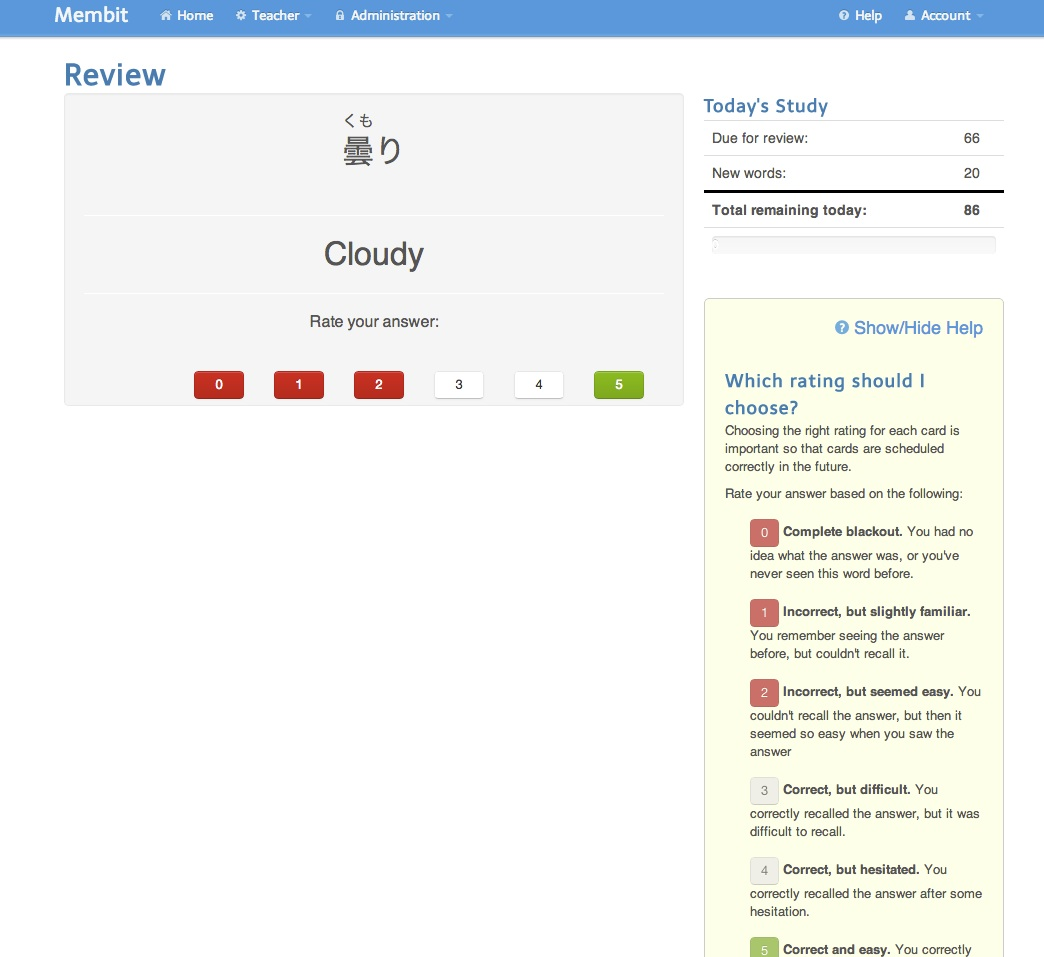
\includegraphics[width=15cm]{appendix/screenshots/review.jpg}}
\caption{Desktop review interface}
\end{figure}

\begin{figure}[h!]
\fbox{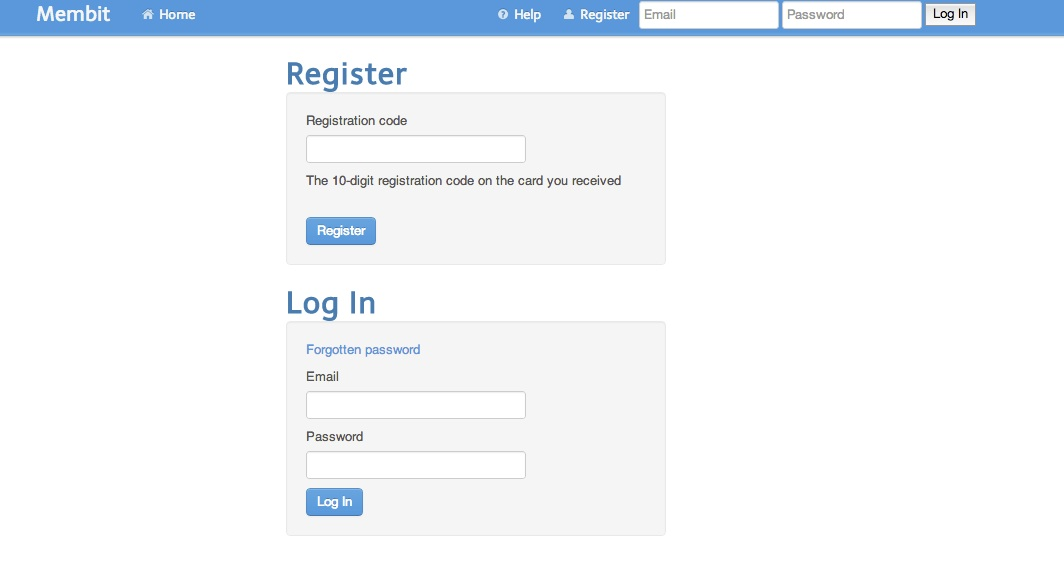
\includegraphics[width=17cm]{appendix/screenshots/login.jpg}}
\caption{Log in screen}
\end{figure}

\chapter{Data}
Data on this CD is also available at \url{https://github.com/jordwest/thesis}
\label{appendix_cd}
\end{document}
